\documentclass[output=paper
,modfonts
,nonflat]{langsci/langscibook} 

\title{Object agreement and grammatical functions: A re-evaluation} 
\author{Peter W. Smith\affiliation{Goethe-Universität, Frankfurt}}

% \chapterDOI{} %will be filled in at production

% \epigram{Khanty}


\abstract{This paper discusses object agreement in the Uralic language Khanty (also known as Ostyak).
The availability of object agreement in this language has been linked \citep{dn2011} to the grammatical function that the object bears, an analysis that if correct, would provide a strong argument in favour of the presence of grammatical functions in Universal Grammar.
I provide a critical re-evaluation of the object agreement data, and show that they can be equally handled in a configurational account.
This paper has further consequences for what constitutes a spell-out domain. 
Following \citet{Baker2015} I argue that differential object marking properties can come about due to the position of the object and what counts as a spell-out domain in that language, which is determined by the strength of the lower phase head v.}

\begin{document}

\maketitle



\section{Introduction} 

One of the fundamental assumptions of the Minimalist Programme, and its predecessor Government and Binding Theory (GB), is that Grammatical Functions such as \textsc{Subject} and \textsc{Object}, whilst they make a great deal of intuitive sense, play no formal role in the grammars that underlie natural language.
This assumption is not universally shared, with the degree to which a framework relies on GFs, differing depending on framework.
Some frameworks are relatively ambivalent on the matter, such as Head Driven Phrase Structure Grammar \citep{pollardsag1994}, whereas in others GFs are a deep and fundamental part of the system, for instance Lexical Functional Grammar (LFG) \citep{dalrymple2001} and Relational Grammar \citep{perlmutterpostal1983}. 

In contrast to these frameworks, the work handled by Grammatical Functions (GFs) in Minimalism/GB has been shifted to other aspects of the theory, notably structural configurations (see \citealt{mccloskey1997} for a detailed overview).
Under this view, the properties that appear to derive from a supposed \subj{} role come instead from the positions in the structure that the subject has passed through.

There is a vast amount of literature that goes to the heart of these questions, far too big for me to even come close to discussing here. However, for the purposes of this paper, I will focus on the claim made in \citet{dn2011} that object agreement in Khanty (also known as Ostyak) is sensitive to the GF of the object.\footnote{Predecessors of this claim can be found in work by Irina Nikolaeva (\citealt{nikolaeva1999,ostyakgrammar,nikolaeva2001}).} 
Specifically, their claim, which I will elaborate on in greater detail below, is that there are two types of objects in Khanty which can be distinguished in terms of their GF: \object{} and \robj, and only the former type of object is able to enter into object agreement in the language.
The appeal to GFs is supported by the clustering of syntactic properties that accompany object agreement.

This paper is organised in the following way. In section \ref{gfagr} I discuss purported cross-linguistic connections between GFs and agreement, before I look at Khanty and the specifics of \citet{dn2011}'s claim in section \ref{Khanty}.
In section \ref{reanalysis} I show that the agreement facts of Khanty can be handled under a theory without referencing GFs, drawing particularly on an analysis of Differential Object Marking effects in \citet{Baker2015} with some minor additions and changes.
However, this leaves a residue of properties to be accounted for, which will be the focus of section \ref{residue}.
I then conclude the paper in section \ref{conclusion}.


\section{Grammatical functions and agreement}\label{gfagr}

\subsection{Subject agreement}

As mentioned earlier, the debate surrounding the status of GFs in grammatical theory is far too complicated and long to go into here, but -- especially in a volume about agreement -- it is worthwhile briefly looking at how the issue relates to agreement.
As \citet{corbett2012gr} carefully notes, whilst GFs can provide a useful heuristic of determining which elements are able to enter into agreement relations in a language, it is not possible to describe all agreement patterns in terms of GFs.
For instance, English looks on the surface like a language where agreement could be characterised as taking place between verb and subject, given that overwhelmingly the subject of the sentence agrees with the verb (assuming that there is verbal agreement).
However, there are known instances where agreement between the verb and subject fails, such as in (\ref{ex:english1}), where the plural subject fails to control plural agreement (see \citealt{pollardsag1994} for discussion on these types of nouns). 
Thus, if we would grant that the \subj{} function exists in the grammar of English, it is not the case that all and only elements with the \subj{} function enter into verbal agreement.

\begin{exe}
\ex \label{ex:english1}
Human resources is on the phone.
\end{exe}

\noindent Putting such cases aside, which constitute exceptions to the general rule, the interesting question is whether GFs should be appealed to in the formulation of agreement rules. 
\citet{Moravcsik1974,moravcsik1978} proposes that the notion of GF plays a role in determining what is able to control agreement in a language and we can formulate implicational statements on the basis of these. 
In short, Moravcsik states that if there is agreement in a language, subjects are always able to be agreement controllers.
If there are two elements that are able to control agreement, it will be subject and object. 
If there are three, it will be subject, object and indirect object. 
\citet{Bobaljik2008} refers to the following as the Moravcsik Hierarchy:

\begin{exe}
\ex
\underline{Moravcsik Hierarchy:}\\
Subject $>$ Object $>$ Indirect Object $>$ Adverb
\end{exe}

\noindent \citeauthor{Bobaljik2008}'s discussion of the Moravcsik Hierarchy is relevant for our purposes, because, as he discusses in detail, in a language with a Nominative-Accusative case alignment, Moravcsik's hierarchy competes with an alternate characterisation of what determines the agreement controller, namely morphological case. 
It will generally be the case that in a Nominative-Accusative alignment, the subject is in nominative case whilst the direct object is in accusative case. 
Thus, we could formulate Moravcsik's hierarchy in these languages in terms of morphological case.

Things become interesting in languages with an Ergative-Absolutive case alignment. In this instance, there is no longer a clear match between GF and morphological case: subjects are sometimes absolutive and sometimes ergative, depending on transitivity. Crucially, \citeauthor{Bobaljik2008} shows that there is no language that will agree with an ergative subject, but not an absolutive object.
That is, whilst there are languages with agreement that is triggered by only absoultive arguments, and languages where agreement is either with absolutive or ergative arguments, there does not seem to exist a language that will agree only and exclusively with subjects.
Thus, framing the rules for subject agreement in terms of morphological case, rather than GF, better captures the cross-linguistically attested patterns. 

\subsection{Differential object agreement}

The question of whether GFs play any role in the grammar is also important for object agreement as well, due to a proposal by \citet{dn2011} who argue for an analysis of object agreement in Khanty that crucially appeals to GFs, which will be the focus of section \ref{Khanty} onwards in this paper.
Their analysis of Khanty forms part of a wider theory of Differential Object Marking (DOM) that is couched in Lexical Functional Grammar, and incorporates the use of GFs. I do not intend to provide a critical discussion of all aspects of \citeauthor{dn2011}'s proposal~-- I could not hope to do credit to their work in the space provided here~-- but I wish to focus on this claim and how it relates to DOM that is expressed through agreement.



Differential object marking refers to the phenomenon where objects are marked with special morphology that signals that the object of a sentence fulfils certain conditions, usually related to specificity and definiteness (though not always, see the discussion of Khanty in section \ref{Khanty}).
This can be illustrated by the following, from Sakha (Turkic).
In (\ref{ex:sakha,Baker2015,126a}), the object is specific, and marked for accusative case, whereas in (\ref{ex:sakha,Baker2015,126b}), the object is non-specific and does not receive case marking.

\begin{exe}
  \ex Sakha, \citet[][126]{Baker2015} \label{ex:sakha,Baker2015,126}
\begin{xlist}
\ex
\gll Masha salamaat-y türgennik sie-te.\\
Masha porridge-{\sc acc} quickly eat-{\sc past.3sgS}\\
\glt `Masha ate the porridge quickly.'  \label{ex:sakha,Baker2015,126a}

\ex
\gll Masha türgennik salamaat sie-te.\\
Masha quickly porridge eat-{\sc past.3sgS}\\
\glt `Masha ate porridge quickly.' \label{ex:sakha,Baker2015,126b}
\end{xlist}
\end{exe}


\noindent Differential Object Agreement (DOA) is clearly related to Differential Object Marking and is plausibly the same phenomenon.
\citeauthor{dn2011} treat it as such, and since I do not wish to take a stance on this here I will follow them in this regard. 
DOA is seemingly less widely attested than DOM, but attested across various unrelated languages nonetheless. 
The difference between DOM and DOA is simply that the marking in DOM is realised on the object itself, usually by a case morpheme, whereas in DOA the special marking is carried on the verb by way of an agreement affix. 
In Ruwund (Bantu, \citealt{woolford2001}) verbs will agree with a specific animate object, but not a non-specific one:\footnote{Woolford notes that object agreement is obligatory with \textsc{Goal} arguments, which is somewhat in accordance with Khanty below.
She gets her examples from \citet[][565]{nash1992}.}

\begin{exe}
\ex Ruwund, \citet[][4]{woolford2001}  \label{ex:ruwund}
\begin{xlist}
\ex
{\gll ku-kimb muntu\\
\textsc{inf}-look.for person\\
\glt `to look for a (any) person'} \label{ex:ruwunda}

\ex
{\gll ku-mu-kimb muntu\\
\textsc{inf-O}-look.for person\\
\glt `to look for a/the person' (with a particular person in mind)}  \label{ex:ruwundb}
\end{xlist}
\end{exe}

\noindent DOM and DOA stand as excellent testing grounds for the existence of GFs, given that they refer specifically to a property of objects, with DOA providing a useful base for testing their role in agreement relations.

GB/Minimalist approaches to DOM, where there is no sense that a function `object' exists, have tended to characterise it as an alternation between different positions for the object in the structure.
The idea, in brief, is that objects that are marked have moved into a higher structural position, which in turn causes or licenses the marking that they carry. Objects that carry the features that are prototypical of DOM (such as being definite or specific) have been documented to move to a higher position than their indefinite or non-specific counterparts \parencite{Diesing1992}. 
If marking is then restricted to higher positions, then we expect definite and specific objects to be marked, but indefinites/non-specific objects not to be.
Such movement accounts are supported by instances whereby marking on the object is clearly correlated with a difference in syntactic position, as can be seen in the Sakha data above: \citeauthor{Baker2015} notes that the accusative morpheme is obligatory in
(\ref{ex:sakha,Baker2015,126a}), where the object appears to the left of the adverb, but impossible in (\ref{ex:sakha,Baker2015,126b}), where the object appears to the right of the adverb, suggesting that movement to a higher position does play a role.


A movement approach has been applied to DOA in \citet{woolford1999,woolford2001}, who accounts for this by assuming that objects that show agreement lie in a higher structural position in the clause than objects that don't agree.
Woolford's analysis for Ruwund, couched within Optimality Theory, proposes exclusion constraints that prevent objects with certain features from remaining within the VP.
For the data in (\ref{ex:ruwundb}), Woolford proposes that the object bears the features [$+$specific,$+$animate], and that there is an exclusion constraint operative in the language that prevents objects from bearing those features from remaining in VP.
 \citeauthor{woolford2001} further proposes that objects that have moved to Spec,AgrOP agree with the verb. 
This, coupled with a general condition of economy (``move only if you need to''), predicts that only objects bearing these features will trigger agreement. 
Whilst there are a couple of shortcomings of Woolford's analysis (for instance, it has been to my mind fairly conclusively demonstrated that Spec-Head agreement is not necessary for agreement to take place; see for instance Long Distance Agreement phenomena, \citealt{polinskypotsdam2001}), the general thrust of Woolford's analysis is consistent with a prominent account of DOM taken in GB/Minimalist approaches: high objects get a special marking (only expressed on the verb) by virtue of moving out of the VP domain.\footnote{One of the criticisms levied against this type of approach is that evidence that movement takes place is often lacking, or it is difficult to determine \citep{dn2011,Baker2015}, and sometimes there is evidence against such movement having taken place \citep{kalinweisser2017}. 
There are a variety of proposals regarding DOM that are not based on the movement account \citep{bossong1991,aissen2003,deswart2007,keinemuller2014,kalin2017}, but a complete overview of the field will take us too far afield from our purpose here. Since my major focus is on the supposed role that GFs play, and I base my account (partly) by appealing to movement, I restrict my attention to this approach.}





\section{Khanty and the properties of objects}\label{Khanty}


Khanty (also known as Ostyak) is a Uralic language spoken in Siberia by around 10,000 people \citep{ethnologue}.
It is a fairly typical member of the Finno-Ugric branch of the Uralic languages, showing a mix of agglutinative and fusional morphology.
There are a variety of different dialects \citep{ostyakgrammar}, but in this paper, all the data comes from \citet{nikolaeva1999}, \citet{nikolaeva2001} and \citet{dn2011}, and so I discuss only the northern dialect.

\subsection{Object agreement in Khanty}\label{khantyprop}

First I outline the relevant properties that are crucial for the discussion.
%For this I draw exclusively on \citet{nikolaeva1999,nikolaeva2001,ostyakgrammar} and \citet{dn2011}.
Khanty has obligatory subject agreement with both intransitive and transitive verbs. 

\begin{exe}
\ex \citet[][142]{dn2011}
\begin{xlist}
\ex
{\gll (ma) je:lən o:məs-l-əm.\\
I at.home sit-\textsc{pres}-\textsc{1sgS}\\
\glt `I am sitting at home.'} \label{ex:ostsubjintrans1}

\ex
{\gll (ma) tam kalaŋ we:l-s-əm.\\
I this reindeer kill-\textsc{past-1sgS}\\
\glt `I killed this reindeer.'} \label{ex:Khantysubjtrans1}
\end{xlist}
\end{exe}

\noindent Object agreement appears to be optionally available for transitives if we compare (\ref{ex:Khantysubjtrans1}) with (\ref{ex:Khantysubjobjtrans1}). Note the vowel change in the agreement suffix. \citet{nikolaeva1999} claims that in this case, where the object is singular, we can view the agreement morpheme as a portmanteau that expresses both subject and object agreement. 

\begin{exe}
  \ex \citet[][142]{dn2011}\\
{\gll (ma) tam kalaŋ we:l-s-e:m.\\
I this reindeer kill-\textsc{past-1sgS.sgO}\\
\glt `I killed this reindeer.'} \label{ex:Khantysubjobjtrans1}
\end{exe}

\noindent Notably, if the number of the object changes to either plural or dual, then a clear object agreement suffix arises.
Only the number of the object is registered on the agreement, not person.
The full paradigm of object marking for the verb \emph{we:r} `make/do' is given in Table \ref{tab:objconj}, with the morpheme carrying object agreement in boldface.\footnote{The form of the verb morphology here is $\sqrt{\textsc{make}}$-\textsc{past}-\textsc{ep}-\textsc{obj}-\textsc{subj}.}

\begin{exe}
\ex \citet[][142-143]{dn2011}
\begin{xlist}
\ex
{\gll (ma) tam kalaŋ-ət we:l-sə-l-am.\\
I this reindeer-\textsc{pl} kill-\textsc{past-PlO-1sgS}\\
\glt `I killed these reindeer.'}

\ex
{\gll (ma) tam kalaŋ-ŋəŋ we:l-sə-ŋil-am.\\
I this reindeer-\textsc{dl} kill-\textsc{past-DlO-1sgS}\\
\glt `I killed these two reindeer.'}

\end{xlist}
\end{exe} \newpage \noindent 



\begin{table}\centering
\caption{\label{tab:objconj}The Objective Conjugation in Khanty \parencite{ostyakgrammar}}
\begin{tabular}{l  l  l l l}
\lsptoprule
\multicolumn{2}{c}{Subject}	&	\multicolumn{3}{c}{Object Number}\\	
Number		&	Person		&	\textsc{Singular}				&	\textsc{Dual}							&	\textsc{Plural}\\
\midrule
\textsc{Singular}	&	1		&	we:r-l-{\bf e:m}					&	we:r-l-ə-{\bf ŋil}-am			&	we:r-l-ə-{\bf l}-am\\
			&	2		&	we:r-l-{\bf e:n}					&	we:r-l-ə-{\bf ŋil}-an			&	we:r-l-ə-{\bf l}-an\\
			&	3		&	we:r-l-ə-{\bf lli}			&	we:r-l-ə-{\bf ŋil}-li			&	we:r-l-ə-{\bf l}-ə-lli\\
\textsc{Dual}	&	1		&	we:r-l-{\bf e:mən}			&	we:r-l-ə-{\bf ŋil}-mən	&	we:r-l-ə-{\bf l}-ə-mən\\
			&	2		&	we:r-l-ə-{\bf lən}		&	we:r-l-ə-{\bf ŋil}-lən	&	we:r-l-ə-{\bf l}-ə-llən\\
			&	3		&	we:r-l-ə-{\bf lən}		&	we:r-l-ə-{\bf ŋil}-lən	&	we:r-l-ə-{\bf l}-ə-llən\\
\textsc{Plural}	&	1		&	we:r-l-{\bf e:w}					&	we:r-l-ə-{\bf ŋil}-uw			&	we:r-l-ə-{\bf l}-uw\\
			&	2		&	we:r-l-{\bf ə-lən}		&	we:r-l-ə-{\bf ŋil}-lən	&	we:r-l-ə-{\bf l}-ə-llen\\
			&	3		&	we:r-l-{\bf e:l}					&	we:r-l-ə-{\bf ŋil}-al			&	we:r-l-ə-{\bf l}-al\\
\lspbottomrule
\end{tabular}

\end{table}

\noindent \citet{nikolaeva1999} carefully shows that neither definiteness nor specificity are the relevant factor that controls object agreement in Khanty.
This can be seen already in the contrast between (\ref{ex:Khantysubjtrans1}) and (\ref{ex:Khantysubjobjtrans1}) above, as well as in (\ref{ex:khantyhouse}).
In both sets of examples, the definiteness and specificity remain constant, but object agreement is not seen in the (a) sentences, but is seen in the (b) ones.

\begin{exe}
\ex \citet[][337]{nikolaeva1999} \label{ex:khantyhouse}
\begin{xlist}
\ex
{\gll ma n\v{a}ŋ-en/n\v{a}ŋ xot-en wan-s-əm.\\
I you-\textsc{acc}/your house-\textsc{2sg} see-\textsc{past-1sgS}\\
\glt `I saw you/your house.'}

\ex
{\gll ma n\v{a}n-en/n\v{a}ŋ xot-en wan-s-e:m.\\
I you-\textsc{acc}/your house-\textsc{2sg} see-\textsc{past-1sgS.sgO}\\
\glt `I saw you/your house.'}

\end{xlist}
\end{exe}

\noindent The determining factor in object agreement is topicality, according to \citet{nikolaeva2001}.  Using corpus data, she shows that object agreement is found overwhelmingly when the object is salient and/or pre-established in the discourse.
Furthermore, objects that agree are existentially presupposed by the speaker.
This trait can be most easily seen by looking at the class of objects that do \emph{not} control agreement.
Objects in focus generally do not control object agreement, as shown in the following,  where the object is a \emph{wh}-item (\ref{ex:focwh}), the object serves as the answer to the question (\ref{ex:focanswer}) (new information in the sense of \citealt{lambrecht1994}), and the object is associated with a focus sensitive particle \emph{only} (\ref{ex:focpart}). 
All of the objects in these sentences fail to trigger object agreement.

\begin{exe}
\ex \citet[][143]{dn2011}
\begin{xlist}
\ex
{\gll u:r-na mati kalaŋ we:l-əs/*we:l-s-əlli?\\
forest-\textsc{loc} which reindeer- kill-\textsc{past.3sgS}/kill-\textsc{past-3sgS.sgO}\\
\glt `Which reindeer did he kill in the forest?'} \label{ex:focwh}

\ex
{\gll u:r-na tam kalaŋ we:l-əs/*we:l-s-əlli.\\
forest-\textsc{loc} this reindeer kill-\textsc{past.3sgS}/kill-\textsc{past-3sgS.sgO}\\
\glt `He killed the reindeer in the forest.'} \label{ex:focanswer}

\ex
{\gll tamxatl tup wul a:n wa:n-s-əm/*wa:n-s-e:m.\\
today only big cup see-\textsc{past-1sgS}/see-\textsc{past-1sgS.sgO}\\
\glt `Today I only saw the/a big cup.'} \label{ex:focpart}
\end{xlist} 
\end{exe}

\noindent Furthermore, non-specific objects do not control agreement.
Note that the object in (\ref{ex:nik200122b}) is crucially \emph{not} in focus: focus in Khanty (as in many head final languages) is associated with an immediately preverbal position. 
In (\ref{ex:nik200122b}), the question word \emph{xal\'{s}a} `how' is in focus, but agreement is still not seen between the verb and the object \emph{mu:tra}.
Thus, it is not that case that the lack of object agreement correlates with the object being in focus.

\begin{exe}
\ex \citet[][20]{nikolaeva2001}\\
{\gll ma mu:tra xal\'{s}a u:\'{s}-l-əm/*u:\'{s}-l-e:m?\\
I miracle how know-\textsc{pres-1sgS}/know-\textsc{pres-1sgS.sgO}\\
\glt `How may I know a miracle?'} \label{ex:nik200122b}
\end{exe}


\noindent \citet{nikolaeva2001}, \citet{dn2011} propose that object agreement is mediated by information structure, and in order for an object to show agreement, it must be interpreted as a topic.\footnote{This is simplifying somewhat.
In actual fact, \citet{nikolaeva2001} argues that agreeing objects are secondary topics, as opposed to subjects which are the primary topic of the sentence.
The distinction between primary and secondary topics is relevant for \cite{nikolaeva2001} and \cite{dn2011}, since the subject GF is assigned the primary topic role, and thus, a coarse notion of topic is not sufficient to draw the line between elements that control object agreement on the verb or not.
Rather, secondary topic is introduced to allow for a distinction between which elements are mapped to \textsc{Object} and which are mapped to \robj, see the discussion in section \ref{sec:otherprops}.
This distinction is not immediately relevant to our purposes here, and I refer the reader to the discussion in these works for further elaboration.}

Yet, this only holds for objects bearing the \theme{} role.
When the object bears the \goal{} or the \causee{} theta role, then object agreement is always obligatory, irrespective of information structure (clearly shown in (\ref{ex:dn201118}) where the causee argument is in focus).\footnote{In a ditransitive construction with a goal argument, the goal argument will control agreement on the verb when the \textsc{theme} is unavailable for agreement, such as being in focus.
This is because Khanty allows only one `primary' object per clause, in the sense that only one object can be unmarked whilst the other must be an oblique.
Khanty thus shows both indirective and secundative alignments in ditransitives (see \citealt{haspelmath2005,Barany2015}).
} 

\begin{exe}
\ex \citet[][149]{dn2011}
\begin{xlist}
\ex
{\gll xoj xollə-ptə-s-li?\\
who cry-\textsc{caus-past-3sgS.sgO}\\
\glt `Whom did he make cry?'} \label{ex:dn201118}

\ex
{\gll ma:ne:m zo:lə-ptə-s-li/*xo:llə-pteə-s.\\
I.\textsc{acc} cry-\textsc{caus-past-3sgS.sgO}/cry-\textsc{caus-past-3sgS}\\
\glt `He made me cry.'} \label{ex:dn201119}

\end{xlist}
\end{exe}

\noindent Similarly, when the \goal{} argument is the (primary) object, then verbal agreement is obligatory, contrasting it with when the \theme{} plays the same role. 
This is observed with the following sentence pair. 

\begin{exe}
\ex \citet[][148]{dn2011}
\begin{xlist}
\ex
{\gll ma a:n Pe:tra e:lti ma-s-e:m/ma-s-əm.\\
I cup Peter to give-\textsc{past-1sgS.sgO}/give-\textsc{past-1sgS}\\
\glt `I gave a/the cup to Peter.'}

\ex
{\gll ma Pe:tra a:n-na ma-s-e:m/*ma-s-əm.\\
I Peter cup-\textsc{loc} give-\textsc{past-1sgS.sgO}/give-\textsc{past-1sgS}\\
\glt `I gave Peter a/the cup.'}
\end{xlist}
\end{exe}

\subsection{Other properties connected to object agreement}
\label{sec:otherprops}

In addition to providing the distribution of where object agreement is necessary and where it is impossible, the ability of triggering object agreement is apparently connected to other syntactic properties.
For these properties, objects that show agreement show a commonality with subjects that is lacking with objects that do not show agreement.
The various properties of objects, and how they compare to subjects, are summarised in Table \ref{tab:gfproperties}.
Objects are divided into two categories to reflect the fact that some objects share properties in common with subjects, but other objects do not.\footnote{Object 1 can be replaced with \textsc{Object}, and Object 2 with \robj, once the reader is familiar with the discussion in section \ref{sec:agreementbygf}.}
 I do not wish to go into the details of all the properties here for space reasons, and I refer the reader to \citet{nikolaeva1999} for further elaboration.
As can be seen, with respect to the phenomena of verbal agreement, control in participial clauses, quantifier float, possessive reflexivisation and possessor topicalisation, subjects and agreeing objects form a natural class to the exclusion of non-agreeing objects.

\begin{table}\centering
	\caption{\label{tab:gfproperties}Properties of subjects and objects in Khanty}
	\begin{tabularx}{\textwidth}{l c c c}
		\lsptoprule
		&	Subjects		&	Object 1				&	Object 2\\	
		\midrule
		Verbal Agreement				&	 \ding{51}		&	 \ding{51}			&	\ding{55}\\
		Control in converbial clauses		&	 \ding{51}		&	\ding{55}			&	\ding{55}\\
		Control in Relative Clauses			&	 \ding{51}		&	\ding{55}			&	\ding{55}\\
		Control across Clauses			&	 \ding{51}		&	\ding{55}			&	\ding{55}\\
		Control in Participial Clauses		&	 \ding{51}		&	 \ding{51}			&	\ding{55}\\
		Quantifier Float				&	 \ding{51}		&	 \ding{51}			&	\ding{55}\\
		Control of Possessive Reflexivisation	& \ding{51}		&	 \ding{51}			&	\ding{55}\\
		Possessor Topicalisation			&	 \ding{51}		&	 \ding{51}			&	\ding{55}\\
		\lspbottomrule
	\end{tabularx}
\end{table}

\noindent For instance, both subjects (\ref{ex:n199926}) and agreeing objects (\ref{ex:n199927}) can enter into the possessor topicalisation construction (where the possessor is split from the possessum), whilst non-agreeing objects cannot (\ref{ex:n199928}):

\begin{exe}
\ex \citet[][346]{nikolaeva1999} \label{ex:n1999possess}
\begin{xlist}
\ex[] {
\gll imi ijolti lik-əl et-əl nawəriŋ pela\\
woman always anger-\textsc{3sg} come-\textsc{past.3sgS} frog to\\
\glt The woman, she is always angry with the frog'\\ (lit: her anger always comes to the frog)} \label{ex:n199926}

\ex[] {
\gll Juwan motta xot-əl k\v{a}\'{s}alə-s-e:m.\\
John before house-\textsc{3sg} see-\textsc{past-1sgS.sgO}\\
\glt `I saw John's house before.'}\label{ex:n199927}

\ex[*] {
\gll Juwan motta xot-əl k\v{a}\'{s}alə-s-əm.\\
John before house-\textsc{3sg} see-\textsc{past-1.sgS}\\
\glt `I saw John's house before.'} \label{ex:n199928}
\end{xlist}
\end{exe}

\noindent I will return to a discussion of these properties in section \ref{residue} below, as well as quantifier float and possessive reflexivisation.



\subsection{Agreement by grammatical function}
\label{sec:agreementbygf}

The challenge posed by the Khanty data as outlined in section \ref{khantyprop} is clear. Khanty shows a fairly typical DOM pattern since some objects are marked and others are not, but it is a system that is only partially based on topicality. 
 On the one hand, \theme s vary according to their information structure role, whilst on the other, \textsc{goals} and \textsc{causees} must obligatorily control agreement, independently of whether they are topics or not.
Furthermore, the ability to control object agreement is linked to a range of other syntactic properties.

The key to the explanation offered by \citet{dn2011} is that objects that agree and ones that do not agree are mapped to different grammatical functions.
To do this, they make use of the restricted object function in LFG, which limits the class of elements that can combine with a particular GF to only those bearing a specified thematic role. 
\citeauthor{dn2011} propose that objects in a sentence come in two types.
Firstly, there is \object, which is unrestricted in terms of which types of semantic roles can be mapped to it. Secondly, there is \robj, which is restricted. 
Whilst the GF \object{} is able to be a controller of agreement on the verb, \robj{} is not (see also \citealt{buttking1996}). 
The key part of the proposal is that the \robj{} function is limited to \theme s, whilst the \object{} function is unrestricted, and places no restriction on the semantic role of the argument that it is mapped to. 
To make the theory complete there is a birectional relationship concerning \theme s and GF: \theme s that are topical cannot be mapped to \robj, and must be mapped to the \object{} function, and themese that are \emph{not} topical must be mapped to \robj, and not \object.
Table \ref{tab:dntabsummary} summarises.

\begin{table}
	\caption{\label{tab:dntabsummary}Summary of how functions are assigned}
	\begin{tabularx}{\textwidth}{XXX}
		\lsptoprule
		Function			&	Thematic Role	&	Information Structure\\
		\midrule
		\multirow{4}{*}{\object}	&	Theme		&	$+$Topic\\
		&	Patient		&	$+$Topic\\
		&	Goal			&	\emph{any}\\
		&	Causee		&	\emph{any}\\
		\midrule
		\multirow{2}{*}{\robj}	&	Theme		&	$-$Topic\\
		&	Patient		&	$-$Topic\\
		\lspbottomrule
	\end{tabularx}
\end{table}

\newpage\noindent To make this clearer, we will consider a couple of examples. Firstly, consider a monotransitive sentence where there is no object agreement. 
The object is non-topical, and in keeping with \citeauthor{dn2011}'s generalisation, it does not trigger object agreement. 
Since the object is a \theme{} in this sentence, and is not topical, it will be mapped to the \robj{} function. The f-structure is given in (\ref{fs:killnontop}).\footnote{Information structural roles are not represented in the following, since it is the GF that is crucially linked to object agreement in Khanty.
There is a separate level of information structure with mappings to f-structure in \citet{dn2011}, which regulates that \textsc{theme}s when topics are assigned to the \robj{} function, but to the \textsc{obj} function when not a topic.
For reasons of space I must gloss over this here, but the f-structures are sufficient to make the point.
For a fuller treatment,  I refer the reader to \citet[][especially ch. 4]{dn2011}.}


\begin{exe}
\ex \citet[][142]{dn2011}
\begin{xlist}
\ex
{\gll (ma) tam kalaŋ we:l-s-əm.\\
I this reindeer kill-\textsc{past-1sgS}\\
\glt `I killed this reindeer.'} \label{ex:Khantysubjtrans}

\ex \label{fs:killnontop}
\begin{avm}
\[ pred 	&	`kill'$<$subj,obj$_{\theta}$$>$\\
subj 		&	\[ pred	&	`pro'\\
			pers		&	1\\
			num		&	sg\]\\
obj$_{\theta}$		&	\[ pred	&	`reindeer'\\
			num		&	sg\]\\
		\]
\end{avm}
\end{xlist}
\end{exe}

\noindent In the corresponding sentence with object agreement, we see that because the object is topical it gets mapped to the \object{} function.

\begin{exe}
\ex \citet[][142]{dn2011}
\begin{xlist}
\ex
{\gll (ma) tam kalaŋ we:l-s-e:m.\\
I this reindeer kill-\textsc{past-1sgS.sgO}\\
\glt `I killed this reindeer.'} \label{ex:Khantysubjobjtrans}

\ex
\begin{avm}
\[ pred 	&	`kill'$<$subj,obj$>$\\
subj 		&	\[ pred	&	`pro'\\
			pers		&	1\\
			num		&	sg\]\\
obj		&	\[ pred	&	`reindeer'\\
			num		&	sg\]\\
		\]
\end{avm}
\end{xlist}
\end{exe}

\noindent Finally, consider a ditransitive construction.
Here, object agreement is obligatory.
Note this time, though, that the \goal{} argument is mapped to the \object{} function, whilst the \theme{} is mapped to an oblique argument.


\begin{exe}
\ex \citet[][148]{dn2011}\\
{\gll ma Pe:tra a:n-na ma-s-e:m/*ma-s-əm.\\
I Peter cup-\textsc{loc} give-\textsc{past-1sgS.sgO}/give-\textsc{past-1sgS}\\
\glt `I gave a/the cup to Peter.'} \label{ex:ditroagreementgf}

\ex
\begin{avm}
\[ pred 	&	`give'$<$subj,obj,obl$>$\\
subj 		&	\[ pred	&	`pro'\\
			pers		&	1\\
			num		&	sg\]\\
obj		&	\[ pred	&	`Peter'\\
			num		&	sg\]\\
obl		&	\[ pred	&	`cup'\\
			num		&	sg\]
			\]
\end{avm}

\end{exe}

\noindent At this point the GFs that are assigned to each of the arguments become crucial.
They do so in the formulation of the agreement affixes for Khanty, which refer specifically to the GF.
A subset of the rules of agreement are given in (\ref{ex:khantyagrrules}).
(\ref{cons:subject1sg}) refers to the agreement affix that expresses only agreement with a 1st person singular \textsc{Subject} (applicable to (\ref{ex:Khantysubjtrans})), (\ref{cons:topicobj}) refers to the agreement affix that expresses agreement with a 1st person singular \textsc{subject} \emph{and} a singular \object{} (applicable to (\ref{ex:Khantysubjobjtrans}) and (\ref{ex:ditroagreementgf})), whilst (\ref{cons:topicplobj}) refers to the agreement affix that expresses agreement with a dual \object.\footnote{See Table \ref{tab:objconj}.}

What is crucial is that there is no affix in the lexicon in Khanty that expresses agreement with \robj.

\begin{exe}
\ex \label{ex:khantyagrrules}
\begin{xlist}
\ex \label{cons:subject1sg}
Agreement specifications for the agreement affix \emph{əm}:\\
($\uparrow$ \textsc{subj pers}) = 1\\
($\uparrow$ \textsc{subj num}) = \textsc{singular}

\ex \label{cons:topicobj}
Agreement specifications for the agreement affix \emph{e:m}:\\
($\uparrow$ \textsc{subj pers}) = 1\\
($\uparrow$ \textsc{subj num}) = \textsc{sg}\\
\textbf{($\uparrow$ \textsc{obj num}) = \textsc{singular} }

\ex \label{cons:topicplobj}
Agreement specification for the agreement affix \emph{ŋil}:\\
\textbf{($\uparrow$ \textsc{obj num}) = \textsc{dual} }
\end{xlist}
\end{exe}

\subsection{Summary}

Given the complexity of the conditions that determine where objects agree, which vary according to both the information structure and thematic interpretation of the argument, the appeal to GFs provides an elegant solution to an extremely complex problem.  
Notably, the theory is able to provide an analysis as to why the agreeing objects show the syntactic properties that they do and why they cluster with subjects in this regard: agreement is just one syntactic property that is linked to the \object{} function (and the \subj{} function) but not the \robj{} function.
The differences between topicalised \theme s and non-topicalised \theme s is because the former are mapped to \object, whilst the latter are mapped to \robj.
Furthermore, given that \robj{} is limited to \theme s, we can see why other thematic roles must obligatorily control object agreement irrespective of their agreement structure: they must get mapped to \object.

\section{Khanty agreement without GFs}\label{reanalysis}

In this section I present a configurational account of object agreement in Khanty that eschews the use of GFs.\footnote{A configurational account is also offered in \citet{barany2016b}.}

\subsection{DOM caused by spell-out domains}

As mentioned above, many GB/Minimalist proposals regarding DOM have appealed to a difference in phrase structural position between the objects that are marked (or here, agreed with), and those that are unmarked (not agreed with).
\citet{Baker2015} discusses DOM in the context of formulating a version of dependent case \citep{Marantz1991}, and specifically proposing that VP may form a domain where dependent case is evaluated. 
If we consider once more the Sakha examples, from above, repeated in (\ref{ex:sakha2,Baker2015,1262}), we see that the difference in marking of the object is dependent on whether the object appears to the right or to the left of the adverb.

\begin{exe}
\ex Sakha, \citet[][126]{Baker2015} \label{ex:sakha2,Baker2015,1262}
\begin{xlist}
\ex
\gll Masha salamaat-y türgennik sie-te.\\
Masha porridge-{\sc acc} quickly eat-{\sc past.3sgS}\\
\glt `Masha ate the porridge quickly.' \label{ex:sakha2,Baker2015,126a}

\ex
\gll Masha türgennik salamaat sie-te.\\
Masha quickly porridge eat-{\sc past.3sgS}\\
\glt `Masha ate porridge quickly.'\label{ex:sakha2,Baker2015,126b}
\end{xlist}
\end{exe}


\noindent \citeauthor{Baker2015} proposes that here, the accusative case appears on the object in (\ref{ex:sakha2,Baker2015,126a}) because the object enters into a dependent case configuration with the subject. 
According to \citeauthor{Baker2015}, dependent accusative case can be assigned only when an argument is c-commanded by another argument within a local domain. 
In (\ref{ex:sakha2,Baker2015,126a}), this happens because the object DP is c-commanded by the subject DP. 
However, in (\ref{ex:sakha2,Baker2015,126b}), though the object DP remains c-commanded by the subject DP, the two are split by a spell-out domain (SOD), that is initiated by the phase head (following the standard view in phase theory that phase heads spell out their complements). 
Crucial here is that dependent case in Sakha cannot be assessed across a Spell-out boundary, and so when the object remains within VP it is the only argument within its domain, and dependent case is unable to be assigned. However, when it moves to Spec,vP it is c-commanded by another argument in its domain, and hence receives dependent case.\footnote{Sakha, like Khanty, is a verb final language, but I represent the trees throughout this paper as left-headed.}

\begin{figure}[!h]
\begin{exe}
\ex Adapted from \citet[][126]{Baker2015}\\
\begin{tikzpicture}[baseline,scale=1]
  \Tree [.TP [.NP$_{\textrm{i}}$ Masha ] [.T$'$ T [.vP [.NP t$_{\textrm{i}}$ ] [.vP [.NP porridge-\textsc{acc} ] [.v$'$ v [.\node(4){VP}; [.AdvP quickly ] [.VP ate [.NP porridge ] ] ] ] ] ] ] ]
  \draw[dashed] ([shift=(1.1cm:2.4cm)]4)  arc (90:180:4cm) node[near start, above]  {SOD}; 

\end{tikzpicture}
\end{exe} \vspace{-0.9cm}
\end{figure}
\newpage\noindent Yet, high movement of objects to receive dependent case cannot be the universal pattern, since there are languages that license a dependent case on all objects, irrespective of specificity, for instance in Cuzco Quechua:

\begin{exe}
\ex Cuzco Quechua, \citet[][146]{Baker2015}\\
\gll Juan wawakuna-man miski-*(ta) qunpuni.\\
Juan children-\textsc{dat} candy-\textsc{acc} give.\textsc{hab.3sS}\\
\glt `Juan gives candy to the children.'
\end{exe}
 
\noindent It is unappealing in these cases to assume that \emph{all} objects in these languages move to a high position, so Baker proposes that the permeability of the spell-out domain varies across languages, such that in some languages like Sakha, a spell-out boundary between two arguments will not allow dependent case relationships to be formed. 
However, in others, the spell-out boundary creates no such inhibition, and arguments that are split by a spell-out boundary can enter into a dependent case relationship. 

As to why the spell-out boundary should be permeable in some languages but not in others, \citeauthor{Baker2015} offers an explanation based on the notion that phase heads can be either \emph{hard} or \emph{soft}. 
If a phase head is hard, then the spell-out domain is blocked off for further syntactic operations. 
On the other hand, if the phase head is soft, the contents remain visible. 
Effectively, DOM effects can arise in a language due to a spell-out boundary not permitting certain operations, such as case relationships, across one another. 
In terms of DOM, these effects arise because certain languages have `hard' boundaries that prevent case configurations being established across them (VP is a case-domain in the terms of Baker).
In the following, I propose that we can utilise this distinction also for agreement, and that -- with qualification -- object agreement in Khanty can be prevented by a spell-out domain created by a hard v head.


\subsection{Spell-out domains and Khanty object agreement}

Recall from above that the object agreement suffix lies between the tense marker and the subject agreement. For concreteness in what follows, I will assume the following clause structure. AgrS is assumed to be the locus of subject agreement, whilst a functional head FP is assumed to be the locus of object agreement.


\begin{exe}
\ex
{[$_{\textrm{AgrSP}}$ Subj [$_{\textrm{AgrS'}}$ AgrS [$_{\textrm{FP}}$  [$_{\textrm{F'}}$ F [$_{\textrm{TP}}$  [$_{\textrm{T'}}$ T [$_{\textrm{vP}}$ {\ldots} ] ] ] ] ] ] ]}
\end{exe}

\noindent Following standard Minimalist assumptions (\citealt{Chomsky2000,Chomsky2001}; \emph{et seq.}), I assume that agreement happens when an \agree{} relationship is established between the probe and a goal. 
Furthermore, I will assume that as a syntactic process, an \agree{} relationship -- like Baker's case domains -- can be disrupted by a hard spell-out boundary. That is, an \agree{} relationship is unable to be established across the boundary of a spell-out domain created by a hard phase head.
I will assume that the v head in Khanty is such a hard phase head, and as such, the contents of its spell-out domain are invisible to further syntactic operations such as \agree.

However, an important qualification is in order here: \citet{Baker2015} assumes that the \emph{entire} spell-out domain is invisible (i.e. the whole VP). However, he leaves open the option of the edge of the spell-out domain remaining visible.\footnote{``I suggest that in some languages everything contained in VP is also considered again in CP, whereas in other languages only something that moves out of VP (\emph{or perhaps to the edge of VP}) is carried forward.'' \parencite[][149]{Baker2015} (emphasis mine - PWS).} 
For reasons that will become clear shortly, I will assume that keeping the edge open is the right approach, and thus the specifier position in the complement of a hard phase boundary remains syntactically visible to higher operations, whilst all other elements within the spell-out domain are closed off. 
To see this graphically, the following tree structure demonstrates the relevant boundary. 
Important for our purposes is that \agree{} relationships can be established in any position above the SOD, including Spec,VP.
To preview the analysis: objects that undergo agreement have moved above the SOD, whereas objects that do not remain beneath it.
 
\begin{exe}
\ex \label{ex:khantyfp}
\begin{tikzpicture}[baseline,scale=1]
\Tree [.{\ldots} {\ldots} [.vP Accessible [.v$'$ v [.VP {Accessible} [.\node(4){V$'$}; V Inaccessible  ] ] ] ] ]
\draw[dashed] ([shift=(1.1cm:3.4cm)]4)  arc (90:180:4cm) node[near start, above]  {SOD};
\end{tikzpicture}
\end{exe}

\noindent Before continuing further, I should offer a short word on case assignment, which I remain agnostic about throughout.
\citet{ostyakgrammar} notes that for lexical nouns, there are three cases in Khanty: nominative, locative and translative.
Pronouns by way of contrast, have three cases: nominative, accusative and locative.
Object agreement is crucially disassociated from case, which can be seen when there is a pronominal object.
In the following, object agreement is both seen and not seen when the object has accusative case.

\begin{exe}
  \ex \citet[][65]{ostyakgrammar}\\
    \gll ma naŋ-e:n wa:n-s-ə-m/wa:n-s-e:m.\\
    I you-\textsc{acc} see-\textsc{past-1sg}/see-\textsc{past-1sgOsg}\\
    \glt `I saw you.' \hfill  \label{ex:lowaccobj}
\end{exe}

\noindent It is clear from such examples that (accusative, at least) case is not intimately connected to agreement in Khanty, and so we should not strive to have them handled by the same mechanism (see \citealt[][ch. 5]{baker2008} for more discussion).
However, such data also pose a problem for what I claim: I propose below that object agreement is possible only if the object moves to Spec,VP (or higher).
Case assignment must be independent of this restriction, given that objects can remain low, as it does by assumption in (\ref{ex:lowaccobj}), but still be able to receive accusative case.

I do not have a fully worked out solution to this issue here, but allow me to sketch a possibility.\footnote{Thanks to András Bárány (p.c.) for pushing me to clarify my assumptions regarding case assignment.}
It is possible that the spell-out domains that I propose here are created \emph{after} the point at which case is assigned.
Specifically, assuming that phases, and by consequence SODs are created dynamically, rather than being statically fixed \citep[see for instance][]{bobaljikwurmbrand2005,bobaljikwurmbrand2013,boskovic2014}, then the merger of v is in the usual case responsible for both the determination and creation of the SOD.
Thus, at the point at which v is merged into the derivation, there is a small window of opportunity where v could license accusative case on the object, before the SOD is created.
To the extent that this is correct, then all that needs to be said is that agreement is not open to the same possibility, in the sense that there must be no possibility for agreement in Khanty to happen before the SOD is created.
Given that the head that is responsible for object agreement is high in the structure, then it seems eminently reasonable that the SOD will not be able to remain open at the relevant stage when agreement happens.

\subsubsection{Monotransitive constructions}

First I will focus on monotransitive constructions involving a \theme{} object.\footnote{I assume the same analysis holds for arguments bearing the \textsc{Patient} role.} 
Recall from above that the difference between the two here is that object agreement is triggered if and only if the \theme{} argument is interpreted as a (secondary) topic.
I will assume that the \theme{} is base generated as the complement of V. 
I further assume that arguments that carry the interpretation of being a topic must move to the left periphery of the lower domain. 
For convenience here I assume that it raises to the specifier of vP.\footnote{However, it could well be the case that there are low information structure positions that merge above vP (\emph{cf.} \citealt{belletti2004,belletti2005a}). The argument bearing the [$+$Topic] feature could then be attracted to this head.}
In the higher position, they are able to be accessed through an \agree{} relation initiated by F.
However, since v is a hard phase head in Khanty, it will create a spell-out boundary that prevents an \agree{} relation being established across it.
Thus object agreement is only possible with a \theme{} that has moved out of its base position into (at least) Spec,vP.\footnote{Note that it is further needed that \theme s cannot move to the edge of VP. Such a movement from the complement to the specifier of the same phrase is widely considered to be too short, and as such would be ruled out through considerations of anti-locality: see \citet{abels2003} and \citet{grohmann2011} and references therein.}
In the tree below, and what follows, a solid arrow indicates an \agree{} relation.

\begin{exe}
	\ex
	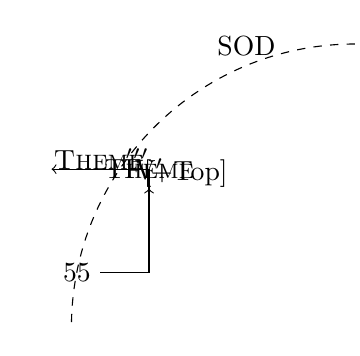
\begin{tikzpicture}[sibling distance=10pt, baseline,scale=0.9]
	% \Tree [.AgrSP Subj [.AgrS' AgrS
	\Tree[.FP \phantom{Text} [.F$'$ \node(p){F}; [.TP \phantom{Text} [.T$'$ T [.vP \node(g){\textsc{Theme}$_{\textrm{[+Top]}}$}; [.v$'$ v [.VP \phantom{Text} [.\node(4){V$'$};  V  \node(t){\textsc{Theme}};  ] ] ] ] ] ] ] ]
	\draw[dashed] ([shift=(1.1cm:3.4cm)]4)  arc (90:180:4cm) node[near start, above]  {SOD} node(bl)[very near end] {\ding{55}}; 
	\draw[->] (p.south) |- (g.west);
	\draw (p.south) |- (bl);
	\draw[dashed,->] (bl) -| (t);
	\end{tikzpicture}
\end{exe} \vspace{-0.2cm}

\noindent This difference in the positioning of \theme s that are interpreted as topics or not is supported by the behaviour of the two regarding floating quantifiers. Nikolaeva argues herself that agreeing objects are VP external and that they do not form a syntactic constituent with the verb based on a variety of tests (see \citealt{nikolaeva1999}, and especially \citealt[][67-69]{ostyakgrammar}). She further shows that quantifier float is possible with objects that show agreement. 
In (\ref{ex:n199924b}), the quantifier \emph{\v{a}sa} `all' can appear either to the left of the object, or to its right. In contrast, when object agreement is absent in (\ref{ex:n199925}), the only possible place for the quantifier is to the left of the argument.
\begin{exe}
\ex \citet[][345]{nikolaeva1999}
\begin{xlist}
\ex 
{\gll l\v{u}w (\v{a}sa) anət (\v{a}sa) il pajət-sə-lli.\\
he all cups all down drop-\textsc{past-3sg.plO}\\
\glt `He dropped all the cups.'} \label{ex:n199924b}

\ex 
{\gll l\v{u}w \v{a}sa anət (*\v{a}sa) il pajt-əs.\\
he all cups all down drop-\textsc{past-3sgS}\\
\glt `He dropped all the cups.'} \label{ex:n199925}
\end{xlist}
\end{exe}

\noindent On the assumption that quantifier float is created when the noun moves away and strands the quantifier (see \citealt{sportiche1988,mccloskey2000,boskovic2004b}) but the position to the right indicates either lack of movement or pied piping of the quantifier, then these data support the account of movement to a higher position. 
In (\ref{ex:n199924b}) the quantifier is either pied piped with, or left behind by, the object when it moves to Spec,vP. However, when there is no movement of the object as in (\ref{ex:n199925}) the quantifier cannot appear to the right of the noun, since there is no step of movement that will strand the quantifier in the original place.\footnote{A point should be made here about \theme{} objects that are in focus, which recall never trigger object agreement.  Khanty is an SOV language which has a preverbal focus position, such that elements that are in focus lie immediately before the verbs. 
This is a fairly common pattern in SOV languages, as \citet{nikolaeva1999} notes, and for this I will follow the proposal of \citet{sener2010} for Turkish, which \citeauthor{sener2010} proposes that this type of language is derived through foci staying \emph{in situ}, and all other elements moving out of the way.
Thus, a \theme{} that is in focus will not move to the left periphery of the lower domain, and hence be unavailable for agreement.}

\subsubsection{Ditransitive constructions and causees}

I now turn attention to \textsc{Goal} arguments. Recall that they obligatorily trigger object agreement when they bear the primary object role in the clause (secundative alignment). 
Regarding the clause structure of Goal arguments in Khanty, I assume that ditransitive constructions in Khanty are formed through a high applicative head (ApplH) \citep{pylkkanen2008} which introduces the goal argument.
On this approach, the \goal{} is introduced in the Specifier of ApplHP. 


\begin{exe}
\ex \label{tree:highappl}
 { [$_{\textrm{vP}}$ {\ldots} [$_{\textrm{v'}}$ v [$_{\textrm{ApplHP}}$ \textsc{Goal} [$_{\textrm{ApplH'}}$ ApplH [$_{\textrm{VP}}$ {} [$_{\textrm{V}}$ V \textsc{Theme}  ] ] ] ] ] ]}

\end{exe}

\noindent Above, we said that \theme s can only trigger object agreement when they are topics, and forced to leave their base position to lie in a position outside the SOD created by v.
%This was enforced by assuming that vP is a hard phase boundary in the sense of \cite{Baker2015}, which causes the VP to be a spell-out domain whose contents (excluding the specifier) are invisible for further computation. 
With the addition of ApplHP, VP is no longer the complement of v, and the spell-out domain becomes every node dominated by ApplH$'$, as shown in (\ref{ex:ditrtree}).\footnote{Note that to save space, irrelevant projections in the tree are omitted here.} 
This draws a line between \goal s and \theme s: the former are introduced in specifiers, whereas the latter are introduced as complements of V. 
If we adopt this, then we keep the insight that agreement is impossible with non-shifted \theme{} arguments since they are within a lower spell-out domain, the edge of a spell-out domain is visible, and hence \goal s will be accessible for agreement.\footnote{For readers who are uncomfortable with the proposal that the edge of the spell-out domain should remain accessible, and that what should be inaccessible ought to be the entirety of what undergoes spell-out (and there are clear conceptual reasons for thinking that this would be the case), there is another option. We could assume that in Khanty ApplHP is a phase in itself \citep{mcginnis2001}, and stipulate the following condition, which would effectively void the spell-out domain status of ApplHP (assuming that phasehood takes preference when (\ref{ex:*phasesod}) applies).
\begin{enumerate}[(i)]
\item A head X cannot head both a phase and a spell-out domain. \label{ex:*phasesod}
\end{enumerate}
This would retain the benefit that v is a hard phase head in Khanty, and always determines that its complement is a spell-out domain. However, there is a loophole just in case that the complement of a phase head is also a phase, and then it would cease to be a spell-out domain. ApplHP fits exactly this, whereas since VP is not a phase head, it will always be a spell-out domain. Yet there are various questions as to why something like (\ref{ex:*phasesod}) should hold in the grammar.}

\begin{exe}
	\ex  \label{ex:ditrtree}
	\begin{tikzpicture}[baseline,scale=1]
	\Tree [.F$'$  \node(p){F}; [. \hspace{0.7cm}{\ldots}\phantom{Text} v [.ApplHP \node(g){\textsc{Goal}}; [.\node(4){ApplH$'$}; ApplH [.VP \phantom{Text} [.V$'$ V \textsc{Theme}  ] ] ] ] ] ]
	%\draw (0.5,-7) to[out=60,in=180] (5,-3);
	\draw[dashed] ([shift=(1.1cm:2.8cm)]4)  arc (90:180:4cm) node[near start, above]  {SOD};
	\draw[->] (p) |- (g);
	\end{tikzpicture}
\end{exe}

\noindent Finally, we turn to causee arguments, which again obligatorily trigger object agreement.
Following \citet{pylkkanen2008} once more, I assume that in causative constructions, there is a \textsc{CausP} that introduces the causation.
Furthermore, I assume that \textsc{Caus} is endowed with an EPP feature that requires something to move into its specifier. Note then that even for verbs that are unaccusative, this means that the internal argument will raise out of the VP and be in a position whereby it can trigger agreement. This arguably relates to the verb \emph{cry}. \citeauthor{dn2011} show that, even when a causee argument is in focus, it will trigger object agreement. 

\begin{exe}
\ex \citet[][149]{dn2011} \label{ex:dnp149}\\
{\gll xoj xo:llə-ptə-s-li?\\
who cry-\textsc{caus-past-3sgS.sgO}\\
\glt `Whom did he make cry?'}
\end{exe}

\noindent The structure for (\ref{ex:dnp149}) is identical to the one given in (\ref{ex:ditrtree}), only ApplHP is replaced by CausP, whose specifier is filled by \emph{xoj}, making it accessible for agreement.

\subsection{Summary and discussion}

In this section I have offered an analysis of the object agreement pattern in Khanty that neither appeals to GFs, nor assumes that there is one given position in the clause that triggers object agreement. 
I will discuss the first point in the next section.
The second point I believe is an interesting step forward. 
As noted above, one of the criticisms levied against movement approaches to DOM is finding evidence for the movement, which is not a problem here, but often it is difficult to define the class of elements that would move to a given position. 
If there is a single characteristic, then it is possible that all elements sharing that feature are attracted to a certain position.
If not, however, then one is always open to the charge of arbitrariness.

Khanty shows exactly this problem, where it is difficult to generate an exact natural class of elements that trigger object agreement on the verb. 
%Given the complex interaction of information structure and thematic role, it is nigh on impossible to find what links all of them.
For instance, if one would only look at \theme s, one could argue that there is a topic position that all agreeing objects lie in.
However, whilst \citet{nikolaeva2001} argues that goals are more prototypically topical than \theme s, and are mapped to the secondary topic role when the direct object is not a topic, such an approach runs into an issue when we consider that focussed causees trigger object agreement.
It seems unlikely that something can be both a focus and a topic at the same time, and so it cannot be the case that topicality is the sole feature that is responsible.
However, under the approach discussed here we do have a link: all elements that trigger object agreement lie either at the edge, or outside the spell-out domain that is caused by v. 
Since v is a hard phase in Khanty (by assumption), then anything which is within this lower domain will not be able to enter into an \agree{} relation with F, and object agreement is impossible.

\section{A residue of object properties}\label{residue}

Up to this point, our interest has been in showing that one can analyse object agreement in Khanty without employing GFs. 
%I believe that I have done so, through an implementation of the `hyrbid' approach to DOM that \citet{Baker2015} employs.
However, simply showing that \emph{agreement} in Khanty can be handled without GFs does not do justice to the approach of \citet{dn2011}.
Recall from Table \ref{tab:gfproperties} above that the arguments that control object agreement on verbs share a number of properties with subjects. 
This paints them in contrast with objects that do not control agreement on verbs, which do not share these properties. 
The strength of \citeauthor{dn2011}'s approach is that it provides an analysis for why this should hold: agreement is just one of the factors that is linked to the \subj{} and \object{} GFs, but not linked to \robj.

Before concluding the paper, it behoves me to discuss these somewhat.\footnote{I will not discuss control in participial clauses, and must leave this for future research.} 
Since I only have the data for these with relation to \theme{} arguments, I will only discuss these, but I do not see anything that would prevent what I propose from carrying over to \textsc{goal}s and \textsc{causee}s too.
In the previous section, I suggested that we can understand the facts of Quantifier Float, given that topicalised \theme s are compelled to move into a higher position in the structure than non-topic \theme s.

This leaves us with two syntactic properties left, both related to possession.
Firstly, \citet{nikolaeva1999} shows that agreeing objects, like subjects, can control possessive reflexivisation, but non-agreeing objects cannot. 

\begin{exe}
\ex \citet[][344]{nikolaeva1999} \label{ex:n1999possessrep}
\begin{xlist}
\ex
{\gll a\'{s}i p\v{o}x-əl reskə-s-li.\\
father son-\textsc{3sg} hit-\textsc{past-3sgS.sgO}\\
\glt `The father\textsubscript{i} hit his\textsubscript{i} son.'}

\ex
{\gll ittam s\v{a}rt k\v{u}tpe-l ewəlt m\v{u}w-na l\v{a}skə-s-li.\\
this pike middle-\textsc{3sg} from ground-\textsc{loc} throw-\textsc{past-3sg.sgO}\\
\glt `He threw this pike\textsubscript{i} to the ground (holding it) in the middle (in its\textsubscript{i} middle).'} \label{ex:n199921}

\ex
{\gll a\'{s}i xot-əl-na p\v{o}x-əl want-əs.\\
father house-\textsc{3sg-loc} son-\textsc{3sg} see-\textsc{past-3sgS}\\
\glt `The father\textsubscript{i} saw his\textsubscript{i} son\textsubscript{k} in his\textsubscript{i/*k} house.'} \label{ex:n199922}

\end{xlist}
\end{exe}

\noindent These data clearly fit in with our approach here. 
Since there is no object agreement in (\ref{ex:n199922}), this is indicative of the \theme{} object not having moved. 
\emph{P\v{o}x-əl} therefore cannot serve as the binder of the reflexive pronoun in the locative, because it does not c-command it.
In contrast, in (\ref{ex:n199921}), the binding relationship is fine because \emph{s\v{a}rt} has moved higher in the clause, and can bind the possessive in the locative.





The second aspect of possession to consider is possessor topicalisation.
Recall that agreeing objects, like subjects, can enter into a possessor topicalisation construction, whilst non-agreeing objects cannot.
Descriptively, the possessor topicalisation construction in Khanty involves the possessor being split from the possessum, as can be seen in the following ((\ref{ex:n1999possess2})=(\ref{ex:n1999possess}b,c)).

\protectedex{
\begin{exe}
	\ex \citet[][346]{nikolaeva1999} \label{ex:n1999possess2}\\
	\gll Juwan motta xot-əl k\v{a}\'{s}alə-s-e:m/*k\v{a}\'{s}alə-s-əm.\\
		 John before house-\textsc{3sg} see-\textsc{past-1sgS.sgO}/see-\textsc{past-1.sgS}\\
	\glt `I saw John's house before.'\label{ex:n1999272}
\end{exe}}


\noindent External possession in this way is exhibited in a range of languages (see the papers in \citealp{paynebarshi1999}), and has invited a range of proposals regarding how it should be accounted for, specifically whether the external possession construction is derived from the regular possessive construction through a raising or a control type analysis (see \citealt{deal2013b} for an overview). 
I will assume a control analysis here, whereby the external possessor controls (through \agree) a PRO that is in the canonical position for possessors.
Specifically, I assume that possessor topicalisation constructions involve the merging of an element in a left-peripheral position, which I take to be (high) Spec,TopP, and this element serves as the binder of PRO.\footnote{\citet{paynebarshi1999b} take external possession to be instances when the possessor assumes a core sentential function, as in the German possessor raising constriction \citep{hole2005}. However, they note that there are instances of topics that act as external possessors, and so I will assume here that external possession is not limited to adding an extra core argument to a verb.
It is of course possible that the external possessor is not in fact generated directly in Spec,TopP, but rather is merged in an \emph{affectee} position in the spine, before raising to Spec,TopP. 
I leave this matter for future research.} 


For objects, however, much depends on the position of the object. I assumed above that topic marked objects move out of the VP. PRO is properly licensed since the \agree{} relation can succeed.
However, note that if PRO is part of an object that has remained low, then it will be unable to be controlled, and the derivation crashes: see the tree in (\ref{tree:objposs}).

\begin{figure}
\begin{exe}
\ex \label{tree:objposs}
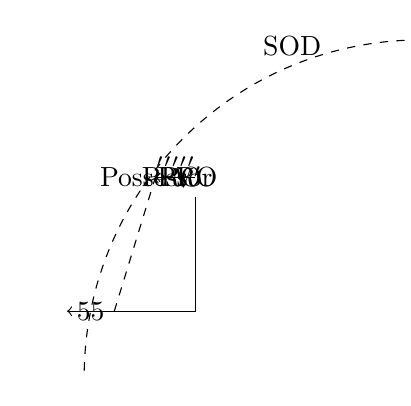
\begin{tikzpicture}[baseline,scale=0.8]
\Tree [.TopP \node(1){Possessor}; [.Top$'$ Top [.AgrSP Subj [.AgrSP$'$ AgrS  [.vP [.PossP \node(2){PRO}; [.Poss$'$ Poss \qroof{...}.NP ] ] [.v$'$ v [.VP \phantom{Text} [.\node(4){V$'$}; V [.PossP \node(7){PRO}; [.Poss$'$ Poss \qroof{...}.NP ] ] ] ] ] ] ] ] ] ]
\draw[->] (1) |- (2.west);
\draw[dashed] ([shift=(1.1cm:4.2cm)]4)  arc (90:180:5.35cm) node[near start, above]  {SOD}  node(bl)[very near end] {\ding{55}};
\draw[->] (1) |- (bl.west);
\draw[->,dashed] (bl.east) to (7.west);
\end{tikzpicture}
\end{exe} \vspace{-0.9cm}
\end{figure}


Whilst assuming the prolepsis account for this construction may seem a bit \emph{ad hoc}, there is in some evidence that is suggestive at least that it may be on the right track. 
\citet[][345]{nikolaeva1999} notes that possessives in Khanty are formed with the possessor to the left of the head noun. 
When the possessor is a possessive pronoun, then there is agreement between the possessor and the possessum, with an affix on the possessum that realises the person and number of the possessor.
When the possessor is a lexical noun, then the order of the possessor and the possessum remains the same, but the agreement is not realised.
I take this to mean that when the possessor is a pronominal element (by which I mean less than a fully lexical R-expression), agreement between the two is obligatory, but not possible when the possessor is a lexical noun. Crucially, in possessor topicalisation, \citeauthor{nikolaeva1999} shows that agreement is \emph{obligatory}, which could be taken as evidence of the presence of PRO in Spec,PossP.  
Thus, we have seen that the current approach can also handle the divergence in behaviour between agreeing objects related to quantifier float, possessor reflexivisation and possessor topicalisation.

\begin{exe}
	\ex
	\begin{tabbing}
		*Ma\v{s}a jernas-əl\hspace{10mm} \= \emph{intended}: `Masha's dress.'\kill
				a.	n\v{a}ŋ jernas-en			\> 	`your dress-\textsc{2sg}'\\
		b.	l\v{u}w jernas-əl 	\>	`his/her dress-\textsc{3sg}'\\
		c.	Ma\v{s}a jernas			\>	 `Masha's dress'\\
		d. 	*Ma\v{s}a jernas-əl	\>	 \emph{intended}: `Masha's dress.'\\
	\end{tabbing} 
\end{exe}

\section{Conclusions}\label{conclusion}

The aim of this paper has been to examine whether it is possible to analyse the facts of Khanty object agreement in a system that does not resort to employing GFs. 
The aim is thus relatively modest, but touches upon key theoretical questions as to what the grammar has, and what it does not have, access to.
I hope to have shown in the discussion in section \ref{reanalysis} that it is possible to capture the facts of agreement in an approach that eschews GFs. 
In doing so, I made qualified use of how DOM effects can arise proposed in \citet{Baker2015}, namely that a hard phase boundary can create a domain low in the structure such that syntactic operations cannot cross it.
All objects that lie structurally above this boundary cause agreement on the verb, and ones that lie beneath do not.

However, what I also hope to have shown is that this approach also allows us an account that links together the other syntactic properties of agreeing and non-agreeing objects.
Linking all of the properties together was a major part of the elegance of \citeauthor{dn2011}'s account and any reanalysis of the Khanty data should strive for this too.
I hope to have convinced the reader that it is not necessary to appeal to GFs to do this: but rather the distinction between \object{} and \robj{} need not be taken to be a theoretical primitive, but falls out from a difference in phrase structure.

There are of course, few if any implications for LFG: it does not in any way show the LFG account to be wrong. 
I do not claim that the current approach should be seen as better than \citeauthor{dn2011}'s approach (nor, I hope, worse), and the analysis given here will do little to sway anyone one way or another on the question of the status of GFs in the grammar.
As noted at the outset, that problem deserves, and has attracted, a far larger discussion, and presumably will for many years to come.
But, I hope that this offering at the very least shows that the complicated facts of Khanty, on close inspection, offer little in favour of evidence for GFs.

\section*{Abbreviations}

\begin{multicols}{2}
	\begin{tabbing}
		\textsc{DOA}\hspace{5mm} \= Differential Object Agreement\kill
		\textsc{abs}\>absolutive\\
		\textsc{acc}\>accusative\\ 
		\textsc{caus}\>causative\\
		\textsc{dat}\>dative\\
		\textsc{DOA}\>Differential Object Agreement\\
		\textsc{DOM}\>Differential Object Marking\\
		\textsc{dl}\>dual\\
		\textsc{ep}\>epenthetic vowel\\
		\textsc{erg}\>ergative\\
		\textsc{GF}\>Grammatical Function\\
		\textsc{hab}\>habitual\\
		\textsc{inf}\>infinitive\\
		\textsc{LFG}\>Lexical Functional Grammar\\
		\textsc{loc}\>locative\\
		\textsc{nom}\>nominative\\
		\textsc{neg}\>negation\\
		O\>object agreement\\
		%\textsc{obj}~=~object,
		\textsc{obl}\>oblique\\
		\textsc{pl}\>plural\\
		\textsc{pres}\>present\\
		S\>subject agreement\\
		SOD\>Spell-out domain\\
		%\textsc{subj}~=~subject
		\textsc{sg}\>singular\\
	\end{tabbing} 
\end{multicols}

\section*{Acknowledgements}

I would like to thank András Bárány, Fenna Bergsma, Katharina Hartmann, Johannes Mursell, Beata Moskal, Zheng Shen and an anonymous reviewer for discussions and comments on this paper.


{\sloppy
\printbibliography[heading=subbibliography,notkeyword=this]
}
\end{document}
